\chapter{Resultados}

\noindent En este último capítulo se analizan los resultados el experimento en ambos ambientes. 

Para cada proceso se registró el tiempo total de ejecución, el tiempo de escritura, el tiempo entre el envío del comando, el tiempo de inicio de la ejecución, el porcentaje de ejecuciones completadas de manera exitosa y cómo estas cantidades escalan al cambiar de ambiente y de número de datos a procesar. A continuación se resumen las conclusiones más importantes sobre el proceso.

Durante esta investigación buscamos conocer la rapidez con la que cada herramienta ejecuta cada tarea pero también cómo cambia esta relación cuando modificamos el número de datos o al cambiar el ambiente de ejecución y así tener una idea de su capacidad de escalamiento. Por otro lado, buscamos ver la consistencia del tiempo de ejecución de los procesos y también conocer qué tan robusto es cada \textit{framework} para determinar si uno es más confiable que el otro para completar las tareas.

\newpage

\section{Ambiente local}

En esta sección primero revisaremos los resultados de cada \textit{framework} en los distintos procesos y a través de las diferentes muestras de datos al ejecutar los procesos en el ambiente local. Después de una revisión individual de cada muestra de datos vamos a pasar a un análisis global en el que analizaremos la capacidad de escalamiento de la herramienta en una computadora local.

En la primera sección nos centraremos en las siguientes características y capacidades de cada \textit{framework} y después se hará una conclusión general para cada muestra de datos. A continuación se listan las características que se evaluarán y en qué consistirá el análisis para determinar el mejor desempeño de una herramienta frente a la otra.

\begin{itemize}
	
	\item \textbf{Robustez} Analizar qué tan resistentes a fallos son los procesos y su confiabilidad para terminar las tareas asignadas. Las principal métrica para evaluar esto será el porcentaje de ejecuciones completadas exitosamente en cada proceso.
	
	\item \textbf{Variación} Medir la variación del tiempo de ejecución de cada proceso en cada \textit{framework} y establecer cuál de los dos es más consistente en el tiempo de ejecución. Para este análisis se utilizará la desviación estándar de el tiempo de duración y el coeficiente de variación como métricas principales.
	
	\item \textbf{Inicio de la ejecución} Comparar el tiempo que le toma a cada proceso ejecutar la primera línea de código. Esto dará una idea de qué tanto tiempo le toma a cada herramienta la asignación de recursos y configuraciones previas a la ejecución del código. La principal métrica para comparar será el tiempo registrado entre la ejecución del comando que inicia el proceso y la primera acción ejecutada dentro del proceso.
	
	\item \textbf{Escritura} Determinar cuál \textit{framework} es más rápido para escribir el resultado a cada destino. Se analizarán de forma separada los procesos que tienen como destino final una base de datos \textit{MySQL} y los que escriben a archivos \texttt{parquet} como destino final. La principal métrica será el tiempo de escritura registrado por cada proceso. Los procesos que escriben a archivos \texttt{parquet} son: \texttt{demoras\_aeropuerto\_destino}, \texttt{demoras\_aerolinea} y \texttt{demoras\_ruta\_aeropuerto}, mientras que los que escriben a \textit{MySQL} son: \texttt{demoras\_aeropuerto\_origen}, \texttt{demoras\_ruta\_mktid}, \texttt{flota} y \texttt{dijkstra}, aunque en caso del último proceso, el resultado escrito raramente es mayor a 5 registros. Por último, el proceso \texttt{elimina\_nulos} imprime su resultado en consola y no será considerado para el análisis de tiempo de escritura.
	
	\item \textbf{Capacidad de cómputo} Establecer qué herramienta tiene un tiempo menor de procesamiento de los datos. El tiempo de cómputo engloba el tiempo de lectura de la fuente de datos, el tiempo de cálculo de resultados y la transferencia de datos necesaria. Este tiempo no incluye el tiempo transcurrido para las tareas de escritura o el tiempo de inicio de la ejecución. La principal métrica será el tiempo total transcurrido, quitando el tiempo de escritura.
	
	\item \textbf{Duración} Contrastar el desempeño de una herramienta frente a la otra en el tiempo total de ejecución de cada proceso. La métrica para comparar los \textit{frameworks} será el tiempo de ejecución registrado en cada proceso y los ratios calculados de la siguiente manera: $\frac{\texttt{tiempo\_de\_ejecucion\_dask}}{\texttt{tiempo\_de\_ejecucion\_spark}}$ y $\frac{\texttt{tiempo\_de\_ejecucion\_spark}}{\texttt{tiempo\_de\_ejecucion\_dask}}$.

	
\end{itemize}

\subsection{Ejecución local con 10,000 registros}

Las conclusiones más relevantes sobre esta muestra de datos son las siguientes:

\begin{center}
\begin{figure}
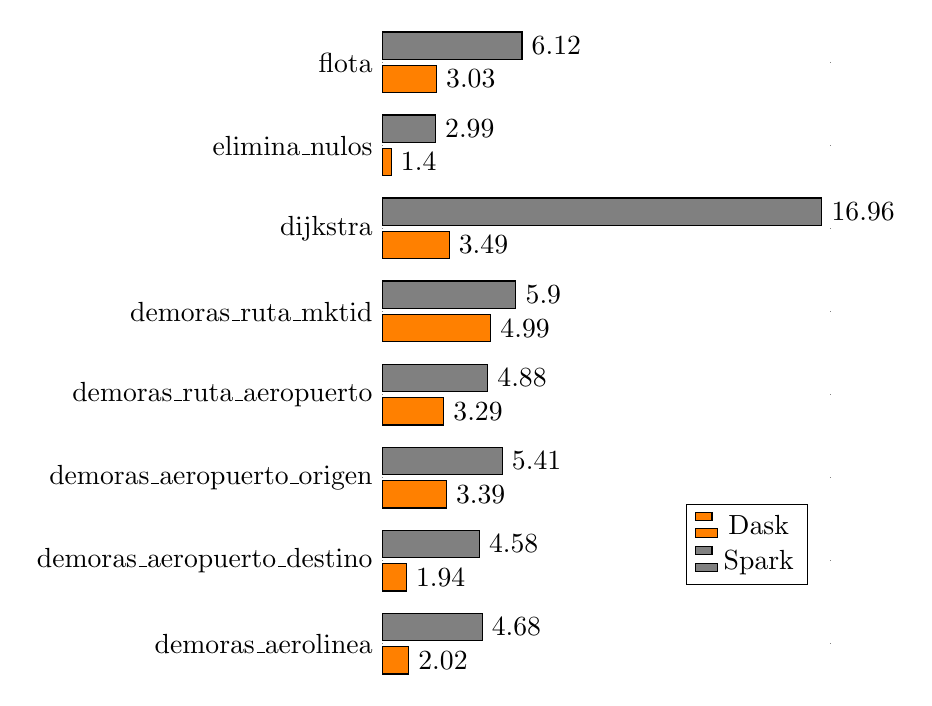
\begin{tikzpicture}
  \begin{axis}[
    xbar,
    y axis line style = { opacity = 0 },
    axis x line       = none,
    y                 = 30,
    x                 = 10,
    legend style={at={(0.95,0.25)}},
    clip              = false,
    tickwidth         = 0.1pt,
    ytick             = data,
    enlarge y limits  = 0.02,
    enlarge x limits  = 0.02,
    symbolic y coords = {demoras\_aerolinea, demoras\_aeropuerto\_destino, demoras\_aeropuerto\_origen, demoras\_ruta\_aeropuerto, demoras\_ruta\_mktid, dijkstra, elimina\_nulos, flota},
    nodes near coords,
  ]
  \addplot[fill=orange] coordinates { (2.024,demoras\_aerolinea)
  						(1.939,demoras\_aeropuerto\_destino)
  						(3.386,demoras\_aeropuerto\_origen)
  						(3.291,demoras\_ruta\_aeropuerto)
  						(4.991,demoras\_ruta\_mktid)
  						(3.488,dijkstra)
  						(1.395,elimina\_nulos)
  						(3.029,flota)};
                         
  \addplot[fill=gray] coordinates { (4.678,demoras\_aerolinea)
  						(4.578,demoras\_aeropuerto\_destino)
  						(5.406,demoras\_aeropuerto\_origen)
  						(4.881,demoras\_ruta\_aeropuerto)
  						(5.901,demoras\_ruta\_mktid)
  						(16.957,dijkstra)
  						(2.993,elimina\_nulos)
  						(6.12,flota)};
  \legend{Dask, Spark}
  \end{axis}
\end{tikzpicture}
\caption{Duración de los procesos con 10,000 registros}
\label{barras:duracion10K}
\end{figure}
\end{center}


\begin{itemize}
	
	\item \textbf{Robustez} Con la muestra de datos más pequeña, ambos \textit{frameworks} lograron completar todos los procesos sin fallas, por lo que su estabilidad es comparable.
	
	\item \textbf{Variación} Para la mayoría de los procesos \textit{Dask} registró un coeficiente de variación mayor que \textit{Spark}, no obstante, hay que considerar que sus tiempos de ejecución fueron menores y casi siempre menores a 5 segundos, por lo que una variación más grande es razonable. La única excepción a lo anterior fue el proceso \texttt{dijkstra} en el que \textit{Spark} tuvo mayor variación a pesar de tener mayor tiempo de ejecución promedio y en el que ambos \textit{frameworks} registraron la mayor variación debido en gran parte a que este proceso calcula una ruta aleatoria en cada ejecución. Además, es importante notar que la mayoría de los coeficientes de variación se mantuvieron por debajo de 0.03 con la excepción de \texttt{dijsktra} y los procesos \texttt{demoras\_ruta\_mktid}, \texttt{demoras\_ruta\_aeropuerto} y \texttt{flota} de \textit{Dask}, de los cuales dos tuvieron un coeficiente mayor a 0.4. 
	
	\item \textbf{Inicio de la ejecución} Una de las diferencias más evidentes entre ambos \textit{frameworks} es el tiempo que tardan en iniciar la ejecución. En el caso de \textit{Spark} este es de al rededor de un segundo, mientras que \textit{Dask} registró un promedio menor a una centésima de segundo en casi todos los casos (con la excepción de \texttt{dijkstra} que es cercano a medio segundo). Es importante notar que el tiempo de inicio de la ejecución fue calculado de forma separada al tiempo de ejecución por lo que no está incluido dentro del mismo.
	
	\item \textbf{Escritura} \textit{Dask} registró un tiempo mucho menor en la escritura a archivos \texttt{parquet} que \textit{Spark} en todos los casos. La diferencia fue de poco menos de un segundo en los tres procesos que tienen como destino final este tipo de archivo. Por otro lado, cuando el destino de escritura es una base de datos \textit{MySQL}, \textit{Dask} también registró un mejor desempeño aunque la diferencia no es tan evidente como en el caso de archivos \texttt{parquet} ya que es de tan solo unas décimas de segundo.
	
	\item \textbf{Capacidad de cómputo} Durante estas ejecuciones, \textit{Dask} registró un tiempo de  cómputo menor en todos los procesos, con una diferencia especialmente evidente en el proceso \texttt{dijkstra} en el que \textit{Spark} fue casi 5 veces más tardado, lo cual sucede debido a que el algoritmo es iterativo y \textit{Dask} tiene una mayor facilidad para utilizar los resultados previos ya que el resultado de cada iteración es un \textit{DataFrame} de \textit{Pandas} almacenado en memoria y \textit{Spark}, por el contrario, tiene como comportamiento predeterminado descartar la información de la ejecución anterior y volver a ejecutar todo el proceso, lo que obliga a utilizar la función \texttt{checkpoint} que escribe los resultados intermedios a disco, lo que puede resultar costoso. Respecto a los otros procesos, a excepción de \texttt{demoras\_ruta\_aeropuerto} y \texttt{demoras\_ruta\_mktid} que involucran la creación de una nueva llave y donde la diferencia en los tiempo de ejecución fue menor a décimas de segundo, \textit{Spark} registró tiempos de casi el doble que los registrados por \textit{Dask}.
	
	\item \textbf{Duración} Al considerar el tiempo de ejecución total, \textit{Dask} también tuvo un mejor desempeño en todos los procesos, especialmente en el proceso \texttt{dijkstra} que fue más de 5 veces más rápido en \textit{Dask}. Por otra parte, los procesos \texttt{demoras\_aerolinea}, \texttt{demoras\_aeropuerto\_destino} y \texttt{demoras\_aeropuerto\_origen} que involucran agregaciones como promedios, obtención del máximo y mínimo y conteos utilizando múltiples llaves para agrupar, tuvieron un tiempo de ejecución al menos 1.5 veces mayor en \textit{Spark} con mayor diferencia en los procesos que tienen \texttt{parquet} como destino. Adicionalmente, los procesos que realizan tareas de preparación de datos como los procesos \texttt{elimina\_nulos} y \texttt{flota} (cuyas tareas son borrado de registros con nulos y eliminación de duplicados respectivamente) también tuvieron un tiempo de ejecución al menos dos veces mayor en \textit{Spark}. Por último, los procesos que involucran agregaciones como promedio y desviación estándar usando una llave nueva generada a partir de columnas existentes (\texttt{demoras\_ruta\_mktid} y \texttt{demoras\_ruta\_aeropuerto}) tuvieron la menor diferencia de tiempo, siendo entre 1 y 1.5 veces mayor en \textit{Spark} que en \textit{Dask}.  
	
\end{itemize}


\begin{table}
    \centering
    \resizebox{\textwidth}{!}{
    \begin{tabular}{|l|c c c c c c c|}
    \hline
        \multicolumn{1}{|p{2.2cm}|}{\centering \textbf{proceso}} & \multicolumn{1}{p{2.2cm}}{\centering \textbf{framework}} & \multicolumn{1}{p{2.2cm}}{\centering \textbf{número de ejecuciones}} & \multicolumn{1}{p{2.2cm}}{\centering \textbf{duración promedio}} & \multicolumn{1}{p{2.2cm}}{\centering \textbf{desviación estándar}} & \multicolumn{1}{p{2.5cm}}{\centering \textbf{coeficiente de variación}} & \multicolumn{1}{p{2.2cm}}{\centering \textbf{$\frac{\texttt{dask}}{\texttt{spark}}$ (duración)}} & \multicolumn{1}{p{2.2cm}|}{\centering \textbf{$\frac{\texttt{spark}}{\texttt{dask}}$ (duración)}} \\ \hline
        demoras\_aerolinea & dask & 100 & 2.024 & 0.048 & 0.024 & 0.433 & 2.311 \\ % \hline
        demoras\_aerolinea & spark & 100 & 4.678 & 0.065 & 0.014 & 0.433 & 2.311 \\ % \hline
        demoras\_aeropuerto\_destino & dask & 100 & 1.939 & 0.043 & 0.022 & 0.424 & 2.361 \\ % \hline
        demoras\_aeropuerto\_destino & spark & 100 & 4.578 & 0.064 & 0.014 & 0.424 & 2.361 \\ % \hline
        demoras\_aeropuerto\_origen & dask & 100 & 3.386 & 0.095 & 0.028 & 0.626 & 1.597 \\ % \hline
        demoras\_aeropuerto\_origen & spark & 100 & 5.406 & 0.132 & 0.024 & 0.626 & 1.597 \\ % \hline
        demoras\_ruta\_aeropuerto & dask & 100 & 3.291 & 1.688 & 0.513 & 0.674 & 1.483 \\ % \hline
        demoras\_ruta\_aeropuerto & spark & 100 & 4.881 & 0.091 & 0.019 & 0.674 & 1.483 \\ % \hline
        demoras\_ruta\_mktid & dask & 100 & 4.991 & 0.252 & 0.05 & 0.846 & 1.182 \\ % \hline
        demoras\_ruta\_mktid & spark & 100 & 5.901 & 0.135 & 0.023 & 0.846 & 1.182 \\ % \hline
        dijkstra & dask & 99 & 3.488 & 2.448 & 0.702 & 0.206 & 4.862 \\ % \hline
        dijkstra & spark & 99 & 16.957 & 14.158 & 0.835 & 0.206 & 4.862 \\ % \hline
        elimina\_nulos & dask & 100 & 1.395 & 0.039 & 0.028 & 0.466 & 2.146 \\ % \hline
        elimina\_nulos & spark & 100 & 2.993 & 0.057 & 0.019 & 0.466 & 2.146 \\ % \hline
        flota & dask & 100 & 3.029 & 1.308 & 0.432 & 0.495 & 2.02 \\ % \hline
        flota & spark & 100 & 6.12 & 0.553 & 0.09 & 0.495 & 2.02 \\ \hline
    \end{tabular}
    \label{table:duracion10K}}
    \caption{Información sobre la duración total con muestra de 10 mil registros.}
\end{table}


\begin{table}
    \centering
    \resizebox{\textwidth}{!}{
    \begin{tabular}{|l|c c c c c|}
    \hline
        \multicolumn{1}{|p{2.2cm}|}{\centering \textbf{proceso}} & \multicolumn{1}{p{2.2cm}}{\centering \textbf{framework}} & \multicolumn{1}{p{2.2cm}}{\centering \textbf{tiempo de inicio}} & \multicolumn{1}{p{2.2cm}}{\centering \textbf{tiempo de cómputo}} & \multicolumn{1}{p{2.2cm}}{\centering \textbf{$\frac{\texttt{dask}}{\texttt{spark}}$ (cómputo)}} & \multicolumn{1}{p{2.2cm}|}{\centering \textbf{$\frac{\texttt{spark}}{\texttt{dask}}$ (cómputo)}} \\ \hline
        demoras\_aerolinea & dask & 0.009 & 1.837 & 1.995 & 0.501 \\ % \hline
        demoras\_aerolinea & spark & 0.97 & 3.665 & 1.995 & 0.501 \\ % \hline
        demoras\_aeropuerto\_destino & dask & 0.009 & 1.744 & 2.08 & 0.481 \\ % \hline
        demoras\_aeropuerto\_destino & spark & 1.084 & 3.627 & 2.08 & 0.481 \\ % \hline
        demoras\_aeropuerto\_origen & dask & 0.009 & 1.743 & 2.068 & 0.483 \\ % \hline
        demoras\_aeropuerto\_origen & spark & 0.957 & 3.605 & 2.068 & 0.483 \\ % \hline
        demoras\_ruta\_aeropuerto & dask & 0.008 & 3.082 & 1.222 & 0.818 \\ % \hline
        demoras\_ruta\_aeropuerto & spark & 0.971 & 3.767 & 1.222 & 0.818 \\ % \hline
        demoras\_ruta\_mktid & dask & 0.008 & 3.294 & 1.196 & 0.836 \\ % \hline
        demoras\_ruta\_mktid & spark & 1.009 & 3.941 & 1.196 & 0.836 \\ % \hline
        dijkstra & dask & 0.503 & 3.324 & 4.938 & 0.203 \\ % \hline
        dijkstra & spark & 1.518 & 16.413 & 4.938 & 0.203 \\ % \hline
        elimina\_nulos & dask & 0.009 & 1.395 & 2.146 & 0.466 \\ % \hline
        elimina\_nulos & spark & 1.023 & 2.993 & 2.146 & 0.466 \\ % \hline
        flota & dask & 0.008 & 1.741 & 2.714 & 0.368 \\ % \hline
        flota & spark & 1.177 & 4.725 & 2.714 & 0.368 \\ \hline
    \end{tabular}
    \label{table:otros10K}}
    \caption{Información sobre tiempo de cómputo e inicio de la ejecución con muestra de 100 mil registros.}
\end{table}

\begin{table}
    \centering
    \resizebox{\textwidth}{!}{
    \begin{tabular}{|l|c c c c c|}
    \hline
        \multicolumn{1}{|p{2.2cm}|}{\centering \textbf{proceso}} & \multicolumn{1}{p{2.2cm}}{\centering \textbf{framework}} & \multicolumn{1}{p{2.2cm}}{\centering \textbf{destino de escritura}} & \multicolumn{1}{p{2.2cm}}{\centering \textbf{tiempo de escritura promedio}} & \multicolumn{1}{p{2.2cm}}{\centering \textbf{número de renglones escritos}} & \multicolumn{1}{p{2.2cm}|}{\centering \textbf{número de columnas escritos}} \\ \hline
        demoras\_aerolinea & spark & parquet & 1.013 & 12135 & 11 \\ % \hline
        demoras\_aerolinea & dask & parquet & 0.187 & 12135 & 11 \\ % \hline
        demoras\_aeropuerto\_destino & spark & parquet & 0.951 & 22144 & 11 \\ % \hline
        demoras\_aeropuerto\_destino & dask & parquet & 0.195 & 22144 & 11 \\ % \hline
        demoras\_aeropuerto\_origen & spark & mysql & 1.801 & 22086 & 11 \\ % \hline
        demoras\_aeropuerto\_origen & dask & mysql & 1.643 & 22086 & 11 \\ % \hline
        demoras\_ruta\_aeropuerto & spark & parquet & 1.114 & 41147 & 11 \\ % \hline
        demoras\_ruta\_aeropuerto & dask & parquet & 0.209 & 41147 & 11 \\ % \hline
        demoras\_ruta\_mktid & spark & mysql & 1.96 & 38909 & 11 \\ % \hline
        demoras\_ruta\_mktid & dask & mysql & 1.697 & 38909 & 11 \\ % \hline
        dijkstra & spark & mysql & 0.544 & Variable & Variable \\ % \hline
        dijkstra & dask & mysql & 0.164 & Variable & Variable \\ % \hline
        elimina\_nulos & spark & sin escritura & NA & NA & NA \\ % \hline
        elimina\_nulos & dask & sin escritura & NA & NA & NA \\ % \hline
        flota & spark & mysql & 1.395 & 12135 & 6 \\ % \hline
        flota & dask & mysql & 1.288 & 12135 & 6 \\ \hline
    \end{tabular}
    \label{table:write10K}}
    \caption{Información sobre tiempo de escritura y tamaño del resultado con muestra de 100 mil registros.}
\end{table}


En resumen, con la muestra de 10,000 registros, \textit{Dask} fue superior en cuatro rubros: primero, el tiempo de ejecución donde \textit{Dask} fue especialmente rápido en la ejecución de tareas de preparación de datos y ejecución del algoritmo, en segundo lugar, el tiempo de cómputo de todos los procesos donde los resultados fueron similares a los tiempos de ejecución global, en tercer lugar, los procesos de escritura donde \textit{Dask} alcanzó una mayor diferencia de tiempo en la escritura a \texttt{parquet} pero también fue más rápido en la escritura a \textit{MySQL} y en último lugar, \textit{Dask} registró tiempos mucho menores en la ejecución del primer comando. Por otro lado, los \textit{frameworks} tuvieron un desempeño comparable en la robustez ya que ambos lograron la ejecución de todos los procesos sin fallas. Por último, \textit{Spark} registró una menor variación que \textit{Dask} en la mayor parte de los procesos, no obstante, no considero que haya información suficiente para asegurar que es más variable debido a la diferencia en los tiempos de ejecución de una herramienta y la otra y los pequeños tiempos de ejecución presentados con esta muestra de datos.


\subsection{Ejecución local con 100,000 registros}

Las siguientes tablas resumen la información más importante obtenida de las ejecuciones y permite establecer las siguientes conclusiones:

%\begin{center}
%\begin{figure}
%\begin{tikzpicture}
%  \begin{axis}[
%    xbar,
%    y axis line style = { opacity = 0 },
%    axis x line       = none,
%    y                 = 30,
%    x                 = 7,
%    legend style={at={(0.95,0.25)}},
%    clip              = false,
%    tickwidth         = 0.1pt,
%    ytick             = data,
%    enlarge y limits  = 0.02,
%    enlarge x limits  = 0.02,
%    symbolic y coords = {demoras\_aerolinea, demoras\_aeropuerto\_destino, demoras\_aeropuerto\_origen, demoras\_ruta\_aeropuerto, demoras\_ruta\_mktid, dijkstra, elimina\_nulos, flota},
%    nodes near coords,
%  ]
%  \addplot[fill=orange] coordinates { (2.422,demoras\_aerolinea)
%  						(2.321,demoras\_aeropuerto\_destino)
%  						(6.275,demoras\_aeropuerto\_origen)
%  						(4.816,demoras\_ruta\_aeropuerto)
%  						(12.429,demoras\_ruta\_mktid)
%  						(5.713,dijkstra)
%  						(1.433,elimina\_nulos)
%  						(3.737,flota)};
%                         
%  \addplot[fill=gray] coordinates { (5.187,demoras\_aerolinea)
%  						(5.107,demoras\_aeropuerto\_destino)
%  						(6.55,demoras\_aeropuerto\_origen)
%  						(6.046,demoras\_ruta\_aeropuerto)
%  						(9.264,demoras\_ruta\_mktid)
%  						(22.62,dijkstra)
%  						(3.048,elimina\_nulos)
%  						(7.16,flota)};
%  \legend{Dask, Spark}
%  \end{axis}
%\end{tikzpicture}
%\caption{Duración de los procesos con 100,000 registros}
%\label{barras:duracion100K}
%\end{figure}
%\end{center}

\begin{itemize}
	\item \textbf{Robustez} Con esta cantidad de datos, ambos \textit{frameworks} tuvieron resultados satisfactorios en la ejecución de sus procesos sin fallos por lo que uno sigue sin superar al otro en este rubro.
	
	\item \textbf{Variación} En esta ejecución, la desviación estándar fue casi siempre menor a 1 segundo en ambos \textit{frameworks} con algunas excepciones. La variación más grande la presentó \textit{Spark} que alcanzó un coeficiente de variación de 1.07 en el proceso \textit{dijkstra}, no obstante, \textit{Dask} tuvo mayor variación en 5 de los 8 procesos. Sin embargo, la mayor parte de las veces los procesos tuvieron un coeficiente de variación menor a 0.04 por lo que, en general, la variación fue pequeña en ambos.
	
	\item \textbf{Inicio de la ejecución} El tiempo de inicio de la ejecución de \textit{Dask} es significativamente menor a \textit{Spark}, ya que el del primero es menor a 0.01 segundos en casi todos los casos (a excepción del proceso \texttt{dijkstra}) y en el caso de \textit{Spark} es de alrededor de 1 segundo en todos los casos, por lo que el comportamiento se mantiene respecto a la muestra anterior.
	
	\item \textbf{Escritura} De acuerdo a los tiempos de escritura, \textit{Spark} fue más rápido en la escritura a \textit{MySQL} en dos de los cuatro procesos que usan este tipo de escritura (haciéndolo en menos del 63\% del tiempo que le tomó a \textit{Dask}) y con un desempeño similar en dos procesos, en uno de los cuales la diferencia fue menor a 0.1 segundos (\texttt{flota}) y en el otro menor a 0.4 segundos (\texttt{dijkstra}). Esto cambió respecto a las ejecuciones con la muestra anterior donde \textit{Dask} fue más rápido. Por otro lado, \textit{Dask} registró un menor tiempo de escritura a archivos \texttt{parquet} (haciéndolo en menos del 30\% del tiempo que le tomó a \textit{Spark}) en todos los procesos lo cual coincide con el comportamiento de la muestra anterior. 
	
	\item \textbf{Capacidad de cómputo} \textit{Dask} logró un menor tiempo de ejecución promedio en prácticamente todos los procesos con la excepción de, \texttt{demoras\_ruta\_aeropuerto} y \texttt{demoras\_ruta\_mktid}, los procesos que generan una nueva llave durante la ejecución y en los que los tiempos fueron tan solo entre 3\% y 8\% mayores que los registrados en \textit{Spark}. Además, se mantuvo la diferencia importante en \texttt{dijkstra} (casi 4 veces más tardado en \textit{Spark}) y los demás procesos registraron tiempos promedio entre 80\% y 176\% mayores a \textit{Dask}.
	
	\item \textbf{Duración} A excepción del proceso \texttt{demoras\_ruta\_mktid}, \textit{Dask} fue superior a \textit{Spark} en cuanto a la rapidez de ejecución de los procesos. Las menores diferencias de tiempo entre ambos \textit{frameworks} se registraron en el proceso \texttt{demoras\_aeropuerto\_origen} que consiste de un conteo y obtención del valor mínimo. La diferencia de tiempo parece estar influenciada por la escritura más rápida de \textit{Spark} a \textit{MySQL}, ya que en el proceso \texttt{demoras\_aeropuerto\_destino} la diferencia se incrementa a pesar de ser un proceso muy similar, con las diferencias de que hace la agregación a partir del aeropuerto de origen y no el de destino, calcula el mínimo en lugar del máximo y escribe a \texttt{parquet} en lugar de \textit{MySQL}. También es importante notar que el proceso \texttt{demoras\_ruta\_aeropuerto} tuvo un mayor tiempo total de ejecución a pesar de que su tiempo de cómputo fue menor, lo que muestra, una vez más, la importancia en la rapidez de escritura. Adicionalmente, el tiempo de ejecución del proceso \texttt{dijkstra} fue casi 4 veces mayor que el de \textit{Spark}.


\end{itemize}

\begin{table}
    \centering
    \resizebox{\textwidth}{!}{
    \begin{tabular}{|l|c c c c c c c|}
    \hline
        \multicolumn{1}{|p{2.2cm}|}{\centering \textbf{proceso}} & \multicolumn{1}{p{2.2cm}}{\centering \textbf{framework}} & \multicolumn{1}{p{2.2cm}}{\centering \textbf{número de ejecuciones}} & \multicolumn{1}{p{2.2cm}}{\centering \textbf{duración promedio}} & \multicolumn{1}{p{2.2cm}}{\centering \textbf{desviación estándar}} & \multicolumn{1}{p{2.5cm}}{\centering \textbf{coeficiente de variación}} & \multicolumn{1}{p{2.2cm}}{\centering \textbf{$\frac{\texttt{dask}}{\texttt{spark}}$ (duración)}} & \multicolumn{1}{p{2.2cm}|}{\centering \textbf{$\frac{\texttt{spark}}{\texttt{dask}}$ (duración)}} \\ \hline
        demoras\_aerolinea & dask & 100 & 2.422 & 1.351 & 0.558 & 0.467 & 2.142 \\ % \hline
        demoras\_aerolinea & spark & 100 & 5.187 & 0.384 & 0.074 & 0.467 & 2.142 \\ % \hline
        demoras\_aeropuerto\_destino & dask & 100 & 2.321 & 0.068 & 0.029 & 0.454 & 2.2 \\ % \hline
        demoras\_aeropuerto\_destino & spark & 100 & 5.107 & 0.089 & 0.017 & 0.454 & 2.2 \\ % \hline
        demoras\_aeropuerto\_origen & dask & 100 & 6.275 & 0.128 & 0.02 & 0.958 & 1.044 \\ % \hline
        demoras\_aeropuerto\_origen & spark & 100 & 6.55 & 0.262 & 0.04 & 0.958 & 1.044 \\ % \hline
        demoras\_ruta\_aeropuerto & dask & 100 & 4.816 & 0.131 & 0.027 & 0.797 & 1.255 \\ % \hline
        demoras\_ruta\_aeropuerto & spark & 100 & 6.046 & 0.093 & 0.015 & 0.797 & 1.255 \\ % \hline
        demoras\_ruta\_mktid & dask & 100 & 12.429 & 0.309 & 0.025 & 1.342 & 0.745 \\ % \hline
        demoras\_ruta\_mktid & spark & 100 & 9.264 & 0.337 & 0.036 & 1.342 & 0.745 \\ % \hline
        dijkstra & dask & 100 & 5.713 & 2.683 & 0.47 & 0.253 & 3.959 \\ % \hline
        dijkstra & spark & 100 & 22.62 & 24.204 & 1.07 & 0.253 & 3.959 \\ % \hline
        elimina\_nulos & dask & 100 & 1.433 & 0.085 & 0.06 & 0.47 & 2.127 \\ % \hline
        elimina\_nulos & spark & 100 & 3.048 & 0.054 & 0.018 & 0.47 & 2.127 \\ % \hline
        flota & dask & 100 & 3.737 & 0.146 & 0.039 & 0.522 & 1.916 \\ % \hline
        flota & spark & 100 & 7.16 & 0.147 & 0.021 & 0.522 & 1.916 \\ \hline
    \end{tabular}
    \label{table:duracion100K}}
    \caption{Información sobre la duración total con muestra de 100 mil registros.}
\end{table}


\begin{table}
    \centering
    \resizebox{\textwidth}{!}{
    \begin{tabular}{|l|c c c c c|}
    \hline
        \multicolumn{1}{|p{2.2cm}|}{\centering \textbf{proceso}} & \multicolumn{1}{p{2.2cm}}{\centering \textbf{framework}} & \multicolumn{1}{p{2.2cm}}{\centering \textbf{tiempo de inicio}} & \multicolumn{1}{p{2.2cm}}{\centering \textbf{tiempo de cómputo}} & \multicolumn{1}{p{2.2cm}}{\centering \textbf{$\frac{\texttt{dask}}{\texttt{spark}}$ (cómputo)}} & \multicolumn{1}{p{2.2cm}|}{\centering \textbf{$\frac{\texttt{spark}}{\texttt{dask}}$ (cómputo)}} \\ \hline
        demoras\_aerolinea & dask & 0.009 & 2.217 & 1.82 & 0.549 \\ % \hline
        demoras\_aerolinea & spark & 1.325 & 4.036 & 1.82 & 0.549 \\ % \hline
        demoras\_aeropuerto\_destino & dask & 0.009 & 2.072 & 1.905 & 0.525 \\ % \hline
        demoras\_aeropuerto\_destino & spark & 0.964 & 3.947 & 1.905 & 0.525 \\ % \hline
        demoras\_aeropuerto\_origen & dask & 0.008 & 2.085 & 1.899 & 0.527 \\ % \hline
        demoras\_aeropuerto\_origen & spark & 1.027 & 3.96 & 1.899 & 0.527 \\ % \hline
        demoras\_ruta\_aeropuerto & dask & 0.008 & 4.34 & 0.965 & 1.036 \\ % \hline
        demoras\_ruta\_aeropuerto & spark & 0.957 & 4.188 & 0.965 & 1.036 \\ % \hline
        demoras\_ruta\_mktid & dask & 0.008 & 5.03 & 0.926 & 1.08 \\ % \hline
        demoras\_ruta\_mktid & spark & 0.986 & 4.658 & 0.926 & 1.08 \\ % \hline
        dijkstra & dask & 0.688 & 5.543 & 3.986 & 0.251 \\ % \hline
        dijkstra & spark & 1.022 & 22.093 & 3.986 & 0.251 \\ % \hline
        elimina\_nulos & dask & 0.009 & 1.433 & 2.127 & 0.47 \\ % \hline
        elimina\_nulos & spark & 0.964 & 3.048 & 2.127 & 0.47 \\ % \hline
        flota & dask & 0.009 & 1.907 & 2.758 & 0.363 \\ % \hline
        flota & spark & 1.019 & 5.259 & 2.758 & 0.363 \\ \hline
    \end{tabular}
    \label{table:otros100K}}
    \caption{Información sobre tiempo de cómputo e inicio de la ejecución con muestra de 100 mil registros.}
\end{table}

\begin{table}
    \centering
    \resizebox{\textwidth}{!}{
    \begin{tabular}{|l|c c c c c|}
    \hline
        \multicolumn{1}{|p{2.2cm}|}{\centering \textbf{proceso}} & \multicolumn{1}{p{2.2cm}}{\centering \textbf{framework}} & \multicolumn{1}{p{2.2cm}}{\centering \textbf{destino de escritura}} & \multicolumn{1}{p{2.2cm}}{\centering \textbf{tiempo de escritura promedio}} & \multicolumn{1}{p{2.2cm}}{\centering \textbf{número de renglones escritos}} & \multicolumn{1}{p{2.2cm}|}{\centering \textbf{número de columnas escritos}} \\ \hline
        demoras\_aerolinea & spark & parquet & 1.151 & 49439 & 11 \\ % \hline
        demoras\_aerolinea & dask & parquet & 0.205 & 49439 & 11 \\ % \hline
        demoras\_aeropuerto\_destino & spark & parquet & 1.16 & 116746 & 11 \\ % \hline
        demoras\_aeropuerto\_destino & dask & parquet & 0.249 & 116746 & 11 \\ % \hline
        demoras\_aeropuerto\_origen & spark & mysql & 2.59 & 116656 & 11 \\ % \hline
        demoras\_aeropuerto\_origen & dask & mysql & 4.19 & 116656 & 11 \\ % \hline
        demoras\_ruta\_aeropuerto & spark & parquet & 1.858 & 297814 & 11 \\ % \hline
        demoras\_ruta\_aeropuerto & dask & parquet & 0.476 & 297814 & 11 \\ % \hline
        demoras\_ruta\_mktid & spark & mysql & 4.606 & 267505 & 11 \\ % \hline
        demoras\_ruta\_mktid & dask & mysql & 7.399 & 267505 & 11 \\ % \hline
        dijkstra & spark & mysql & 0.527 & Variable & Variable \\ % \hline
        dijkstra & dask & mysql & 0.17 & Variable & Variable \\ % \hline
        elimina\_nulos & spark & sin escritura & NA & NA & NA \\ % \hline
        elimina\_nulos & dask & sin escritura & NA & NA & NA \\ % \hline
        flota & spark & mysql & 1.901 & 49439 & 6 \\ % \hline
        flota & dask & mysql & 1.83 & 49439 & 6 \\ \hline
    \end{tabular}
    \label{table:write100K}}
    \caption{Información sobre tiempo de escritura y tamaño del resultado con muestra de 100 mil registros.}
\end{table}

En conclusión, para esta muestra de datos, \textit{Dask} mantuvo el mejor desempeño en cuatro rubros: primero, el tiempo de ejecución que no mantuvo en todos los procesos pero sí en 7 de 8, después, en el tiempo de cómputo donde fue superado por \textit{Spark} en 2 casos pero mantuvo el resto, en tercer lugar, el tiempo de escritura a archivos \texttt{parquet} donde fue más rápido en todos los casos y con un margen considerable, y en cuarto lugar el tiempo de inicio de la ejecución que fue muy similar al de la muestra anterior. Por otro lado, \textit{Spark} fue superior en la escritura a \textit{MySQL} en dos de los procesos y en los otros tuvo un desempeño similar a \textit{Dask}. Además, \textit{Spark} tuvo una menor variación en muchos de los procesos pero en ambos \textit{frameworks} fue pequeña. Por último, ambas herramientas parecen ser igual de robustas ya que no tuvieron errores con este número de datos. 


\subsection{Ejecución local con 1,000,000 de registros}

De esta ejecución podemos obtener las siguientes conclusiones:

%\begin{center}
%\begin{figure}
%\begin{tikzpicture}
%  \begin{axis}[
%    xbar,
%    y axis line style = { opacity = 0 },
%    axis x line       = none,
%    y                 = 30,
%    x                 = 2,
%    legend style={at={(0.95,0.25)}},
%    clip              = false,
%    tickwidth         = 0.1pt,
%    ytick             = data,
%    enlarge y limits  = 0.02,
%    enlarge x limits  = 0.02,
%    symbolic y coords = {demoras\_aerolinea, demoras\_aeropuerto\_destino, demoras\_aeropuerto\_origen, demoras\_ruta\_aeropuerto, demoras\_ruta\_mktid, dijkstra, elimina\_nulos, flota},
%    nodes near coords,
%  ]
%  \addplot[fill=orange] coordinates { (3.629,demoras\_aerolinea)
%  						(4.617,demoras\_aeropuerto\_destino)
%  						(16.611,demoras\_aeropuerto\_origen)
%  						(17.721,demoras\_ruta\_aeropuerto)
%  						(55.405,demoras\_ruta\_mktid)
%  						(31.371,dijkstra)
%  						(1.817,elimina\_nulos)
%  						(6.57,flota)};
%                         
%  \addplot[fill=gray] coordinates { (6.363,demoras\_aerolinea)
%  						(7.137,demoras\_aeropuerto\_destino)
%  						(11.607,demoras\_aeropuerto\_origen)
%  						(12.019,demoras\_ruta\_aeropuerto)
%  						(49.728,demoras\_ruta\_mktid)
%  						(69.953,dijkstra)
%  						(3.365,elimina\_nulos)
%  						(8.932,flota)};
%  \legend{Dask, Spark}
%  \end{axis}
%\end{tikzpicture}
%\caption{Duración de los procesos con 1,000,000 de registros}
%\label{barras:duracion1M}
%\end{figure}
%\end{center}

\begin{itemize}
	\item \textbf{Robustez} Ambos procesos lograron terminar el 100\% de sus ejecuciones por lo que siguen siendo igual de confiables.
	
	\item \textbf{Variación} En estas ejecuciones \textit{Dask} tuvo una variación mayor en 4 de los 8 procesos con diferencias pequeñas respecto a \textit{Spark}. Una vez más, el proceso con mayor variación para \textit{Spark} fue \texttt{dijkstra} con un coeficiente de variación de 1.344 y con todos los demás menores a 0.06. \textit{Dask}, por su parte, tuvo dos procesos con coeficiente mayor a 0.14 siendo \texttt{demoras\_aeropuerto\_destino} el proceso con mayor variación con un coeficiente de 0.289.
	
	\item \textbf{Inicio de la ejecución} En esta muestra \textit{Spark} presentó un incremento en el tiempo de inicio de la ejecución mientras que \textit{Dask} mantuvo un comportamiento similar a muestras previas. 
	
	\item \textbf{Escritura} La superioridad de \textit{Dask} en la velocidad de escritura a \texttt{parquet} se mantuvo respecto a la muestra anterior, mientras que la superioridad de escritura de \textit{Spark} a \textit{MySQL} se reduce respecto a la muestra anterior ya que sólo es más rápido en dos de los procesos: primero en \texttt{demoras\_aeropuerto\_origen} donde el tiempo de escritura es de casi la mitad del tiempo que el de \textit{Dask}, y en segundo lugar el proceso \texttt{flota} donde la diferencia es mínima, además, la diferencia en el proceso \texttt{demoras\_ruta\_aeropuerto} es mucho menor y favorable a \textit{Dask} cuando en la muestra pasada \textit{Spark} había sido significativamente más rápido. 
	
	\item \textbf{Capacidad de cómputo} Al igual que en la muestra anterior, \textit{Spark} fue más rápido sólo en los procesos \texttt{demoras\_ruta\_aeropuerto} y \texttt{demoras\_ruta\_mktid} en los que \textit{Dask} alcanzó tiempos entre 80\% y 148\% mayores. En \texttt{dijkstra}, \textit{Dask} mantuvo un desempeño mayor aunque sparj fue sólo un 123\% más tardado lo cual es una mejora importante respecto a los resultados de la muestra anterior, sin embargo la necesidad de \textit{Spark} de escribir a disco en cada ejecución sigue dándole una amplia ventaja a \textit{Dask}. Por último, los otros procesos también tuvieron una mejora por parte de \textit{Spark} donde la duración fue entre 29\% y 58\% mayor que es considerable pero mucho menor a las diferencias observadas anteriormente.
	
	\item \textbf{Duración} A pesar de los puntos anteriores, \textit{Spark} redujo la diferencia en el ratio de duración de tiempo en todos los procesos y es más rápido que \textit{Dask} en tres de ellos (\texttt{demoras\_aeropuerto\_origen}, \texttt{demoras\_ruta\_aeropuerto} y \texttt{demoras\_ruta\_mktid}), dos más que en la ejecución anterior. Además, la diferencia en el tiempo de ejecución se redujo a menos del 80\% en todos los procesos (a excepción de \texttt{dijkstra}), cuando en la ejecución pasada muchos fueron más de 100\% más tardados.

\end{itemize}

\begin{table}
    \centering
    \resizebox{\textwidth}{!}{
    \begin{tabular}{|l|c c c c c c c|}
    \hline
        \multicolumn{1}{|p{2.2cm}|}{\centering \textbf{proceso}} & \multicolumn{1}{p{2.2cm}}{\centering \textbf{framework}} & \multicolumn{1}{p{2.2cm}}{\centering \textbf{número de ejecuciones}} & \multicolumn{1}{p{2.2cm}}{\centering \textbf{duración promedio}} & \multicolumn{1}{p{2.2cm}}{\centering \textbf{desviación estándar}} & \multicolumn{1}{p{2.5cm}}{\centering \textbf{coeficiente de variación}} & \multicolumn{1}{p{2.2cm}}{\centering \textbf{$\frac{\texttt{dask}}{\texttt{spark}}$ (duración)}} & \multicolumn{1}{p{2.2cm}|}{\centering \textbf{$\frac{\texttt{spark}}{\texttt{dask}}$ (duración)}} \\ \hline
        demoras\_aerolinea & dask & 100 & 3.629 & 0.06 & 0.017 & 0.57 & 1.753 \\ % \hline
        demoras\_aerolinea & spark & 100 & 6.363 & 0.093 & 0.015 & 0.57 & 1.753 \\ % \hline
        demoras\_aeropuerto\_destino & dask & 100 & 4.617 & 1.337 & 0.289 & 0.647 & 1.546 \\ % \hline
        demoras\_aeropuerto\_destino & spark & 100 & 7.137 & 0.418 & 0.058 & 0.647 & 1.546 \\ % \hline
        demoras\_aeropuerto\_origen & dask & 100 & 16.611 & 0.205 & 0.012 & 1.431 & 0.699 \\ % \hline
        demoras\_aeropuerto\_origen & spark & 100 & 11.607 & 0.488 & 0.042 & 1.431 & 0.699 \\ % \hline
        demoras\_ruta\_aeropuerto & dask & 100 & 17.721 & 0.584 & 0.033 & 1.474 & 0.678 \\ % \hline
        demoras\_ruta\_aeropuerto & spark & 100 & 12.019 & 0.196 & 0.016 & 1.474 & 0.678 \\ % \hline
        demoras\_ruta\_mktid & dask & 100 & 55.405 & 0.564 & 0.01 & 1.114 & 0.898 \\ % \hline
        demoras\_ruta\_mktid & spark & 100 & 49.728 & 0.851 & 0.017 & 1.114 & 0.898 \\ % \hline
        dijkstra & dask & 100 & 31.371 & 4.527 & 0.144 & 0.448 & 2.23 \\ % \hline
        dijkstra & spark & 100 & 69.953 & 94.048 & 1.344 & 0.448 & 2.23 \\ % \hline
        elimina\_nulos & dask & 100 & 1.817 & 0.039 & 0.021 & 0.54 & 1.852 \\ % \hline
        elimina\_nulos & spark & 100 & 3.365 & 0.043 & 0.013 & 0.54 & 1.852 \\ % \hline
        flota & dask & 100 & 6.57 & 0.093 & 0.014 & 0.736 & 1.36 \\ % \hline
        flota & spark & 100 & 8.932 & 0.175 & 0.02 & 0.736 & 1.36 \\ \hline
    \end{tabular}
    \label{table:duracion1M}}
    \caption{Información sobre la duración total con muestra de 1 millón de registros.}
\end{table}


\begin{table}
    \centering
    \resizebox{\textwidth}{!}{
    \begin{tabular}{|l|c c c c c|}
    \hline
        \multicolumn{1}{|p{2.2cm}|}{\centering \textbf{proceso}} & \multicolumn{1}{p{2.2cm}}{\centering \textbf{framework}} & \multicolumn{1}{p{2.2cm}}{\centering \textbf{tiempo de inicio}} & \multicolumn{1}{p{2.2cm}}{\centering \textbf{tiempo de cómputo}} & \multicolumn{1}{p{2.2cm}}{\centering \textbf{$\frac{\texttt{dask}}{\texttt{spark}}$ (cómputo)}} & \multicolumn{1}{p{2.2cm}|}{\centering \textbf{$\frac{\texttt{spark}}{\texttt{dask}}$ (cómputo)}} \\ \hline
        demoras\_aerolinea & dask & 0.008 & 3.381 & 1.518 & 0.659 \\ % \hline
        demoras\_aerolinea & spark & 5.545 & 5.132 & 1.518 & 0.659 \\ % \hline
        demoras\_aeropuerto\_destino & dask & 0.009 & 4.12 & 1.294 & 0.773 \\ % \hline
        demoras\_aeropuerto\_destino & spark & 0.977 & 5.331 & 1.294 & 0.773 \\ % \hline
        demoras\_aeropuerto\_origen & dask & 0.009 & 4.038 & 1.31 & 0.763 \\ % \hline
        demoras\_aeropuerto\_origen & spark & 3.144 & 5.291 & 1.31 & 0.763 \\ % \hline
        demoras\_ruta\_aeropuerto & dask & 0.008 & 15.885 & 0.403 & 2.482 \\ % \hline
        demoras\_ruta\_aeropuerto & spark & 3.769 & 6.401 & 0.403 & 2.482 \\ % \hline
        demoras\_ruta\_mktid & dask & 0.009 & 17.364 & 0.531 & 1.882 \\ % \hline
        demoras\_ruta\_mktid & spark & 3.95 & 9.228 & 0.531 & 1.882 \\ % \hline
        dijkstra & dask & 1.975 & 31.12 & 2.23 & 0.448 \\ % \hline
        dijkstra & spark & 7.847 & 69.412 & 2.23 & 0.448 \\ % \hline
        elimina\_nulos & dask & 0.009 & 1.817 & 1.852 & 0.54 \\ % \hline
        elimina\_nulos & spark & 1.093 & 3.365 & 1.852 & 0.54 \\ % \hline
        flota & dask & 0.009 & 4.389 & 1.574 & 0.635 \\ % \hline
        flota & spark & 0.951 & 6.908 & 1.574 & 0.635 \\ \hline
    \end{tabular}
    \label{table:otros1M}}
    \caption{Información sobre tiempo de cómputo e inicio de la ejecución con muestra de 1 millón de registros.}
\end{table}

\begin{table}
    \centering
    \resizebox{\textwidth}{!}{
    \begin{tabular}{|l|c c c c c|}
    \hline
        \multicolumn{1}{|p{2.2cm}|}{\centering \textbf{proceso}} & \multicolumn{1}{p{2.2cm}}{\centering \textbf{framework}} & \multicolumn{1}{p{2.2cm}}{\centering \textbf{destino de escritura}} & \multicolumn{1}{p{2.2cm}}{\centering \textbf{tiempo de escritura promedio}} & \multicolumn{1}{p{2.2cm}}{\centering \textbf{número de renglones escritos}} & \multicolumn{1}{p{2.2cm}|}{\centering \textbf{número de columnas escritos}} \\ \hline
        demoras\_aerolinea & spark & parquet & 1.231 & 76717 & 11 \\ % \hline
        demoras\_aerolinea & dask & parquet & 0.248 & 76717 & 11 \\ % \hline
        demoras\_aeropuerto\_destino & spark & parquet & 1.806 & 436411 & 11 \\ % \hline
        demoras\_aeropuerto\_destino & dask & parquet & 0.497 & 436411 & 11 \\ % \hline
        demoras\_aeropuerto\_origen & spark & mysql & 6.316 & 436681 & 11 \\ % \hline
        demoras\_aeropuerto\_origen & dask & mysql & 12.573 & 436681 & 11 \\ % \hline
        demoras\_ruta\_aeropuerto & spark & parquet & 5.618 & 1619826 & 11 \\ % \hline
        demoras\_ruta\_aeropuerto & dask & parquet & 1.836 & 1619826 & 11 \\ % \hline
        demoras\_ruta\_mktid & spark & mysql & 40.5 & 1430282 & 11 \\ % \hline
        demoras\_ruta\_mktid & dask & mysql & 38.041 & 1430282 & 11 \\ % \hline
        dijkstra & spark & mysql & 0.541 & Variable & Variable \\ % \hline
        dijkstra & dask & mysql & 0.251 & Variable & Variable \\ % \hline
        elimina\_nulos & spark & sin escritura & NA & NA & NA \\ % \hline
        elimina\_nulos & dask & sin escritura & NA & NA & NA \\ % \hline
        flota & spark & mysql & 2.024 & 76717 & 6 \\ % \hline
        flota & dask & mysql & 2.181 & 76717 & 6 \\ \hline
    \end{tabular}
    \label{table:write1M}}
    \caption{Información sobre tiempo de escritura y tamaño del resultado con muestra de 1 millón de registros.}
\end{table}

En conclusión, podemos ver que al incrementar la muestra de datos la superioridad de \textit{Spark} en la escritura a \textit{MySQL} que parecía existir anteriormente no es tan clara, pero se acentúa su mejor desempeño al operar con una nueva llave. Por otro lado, \textit{Dask} aún conserva la ventaja de la escritura a \texttt{parquet} y es más rápido en la ejecución del proceso (sin contar el tiempo de escritura) en todos los procesos que no requieren de la creación de una nueva llave pero la ventaja respecto a \textit{Spark} se redujo significativamente, esto es especialmente evidente al ver el tiempo de cómputo. En cuanto a la robustez y variación, ambos \textit{frameworks} tienen resultados similares con \textit{Spark} siendo un poco más consistente en la duración de sus ejecuciones. Por último, en el algoritmo iterativo \textit{Dask} sigue teniendo mejor desempeño gracias a su capacidad de mantener en memoria resultados intermedios.

\subsection{Ejecución local con 10,000,000 registros}

%\begin{center}
%\begin{figure}
%\begin{tikzpicture}
%  \begin{axis}[
%    xbar,
%    y axis line style = { opacity = 0 },
%    axis x line       = none,
%    y                 = 30,
%    x                 = 2,
%    legend style={at={(0.95,0.25)}},
%    clip              = false,
%    tickwidth         = 0.1pt,
%    ytick             = data,
%    enlarge y limits  = 0.02,
%    enlarge x limits  = 0.02,
%    symbolic y coords = {demoras\_aerolinea, demoras\_aeropuerto\_destino, demoras\_aeropuerto\_origen, demoras\_ruta\_aeropuerto, demoras\_ruta\_mktid, dijkstra, elimina\_nulos, flota},
%    nodes near coords,
%  ]
%  \addplot[fill=orange] coordinates { (8.604,demoras\_aerolinea)
%  						(11.123,demoras\_aeropuerto\_destino)
%  						(38.7,demoras\_aeropuerto\_origen)
%  						(93.087,demoras\_ruta\_aeropuerto)
%  						(49.728,demoras\_ruta\_mktid)
%  						(135.123,dijkstra)
%  						(1.817,elimina\_nulos)
%  						(6.57,flota)};
%                         
%  \addplot[fill=gray] coordinates { (6.363,demoras\_aerolinea)
%  						(7.137,demoras\_aeropuerto\_destino)
%  						(11.607,demoras\_aeropuerto\_origen)
%  						(12.019,demoras\_ruta\_aeropuerto)
%  						(49.728,demoras\_ruta\_mktid)
%  						(69.953,dijkstra)
%  						(3.365,elimina\_nulos)
%  						(8.932,flota)};
%  \legend{Dask, Spark}
%  \end{axis}
%  \coordinate (A) at (1.6,4.15)
%  \node at (A) {Error de memoria}
%\end{tikzpicture}
%\caption{Duración de los procesos con 10,000,000 de registros}
%\label{barras:duracion10M}
%\end{figure}
%\end{center}

\begin{itemize}

	\item \textbf{Robustez} En la ejecución de los procesos con esta muestra de datos \textit{Dask} presentó problemas en de falta de memoria en las ejecuciones del proceso \texttt{demoras\_ruta\_mktid} por lo que no completó ninguna de las 100 ejecuciones, algo similar se registró en \cite{comparative-evolution} con un ambiente parecido. El problema de memoria aparece cuando \textit{Dask} calcula el resultado final y lo intenta escribir a \textit{MySQL}. Por el contrario, \textit{Spark} completó el 100\% de las ejecuciones en todos los procesos, por lo que parece escalar de forma más estable y tener una mejor administración del uso de recursos.
	
	\item \textbf{Variación} El coeficiente de variación es menor para \textit{Dask} en todos los procesos, por lo que este \textit{framework} es más consistente en sus tiempos de ejecución. Sin embargo, en ambos \textit{frameworks}, el coeficiente es menor a 0.2 en la mayoría de los procesos y las excepciones corresponden a dos procesos de \textit{Spark}: \texttt{dijkstra}, que varía ya que calcula una ruta elegida de forma aleatoria en cada ejecución, y \texttt{elimina\_nulos}, el proceso de menor duración y cuya variación es menor a dos décimas de segundo para \textit{Dask} y menor a 1 segundo para \textit{Spark}, lo que explica el valor alto del coeficiente.
	
	\item \textbf{Inicio de la ejecución} A excepción del proceso \texttt{dijkstra}, el tiempo de inicio de la ejecución sigue siendo mucho menor para \textit{Dask}.
	
	\item \textbf{Escritura} \textit{Dask} mantiene tiempos menores a los registrados por \textit{Spark} en la escritura de datos a archivos \texttt{parquet}. Por otro lado, \textit{Spark} sigue teniendo un tiempo de escritura menor a \textit{MySQL} en el proceso \texttt{demoras\_aeropuerto\_origen} y un tiempo similar los procesos \texttt{dijkstra} y \texttt{flota}. Del proceso \textit{demoras\_ruta\_mktid} no tenemos información para comparar. 
	
	\item \textbf{Capacidad de cómputo} Al ver el tiempo de cómputo, vemos que a \textit{Dask} le toma cerca de 17\% más tiempo completar el cálculo de los procesos \texttt{demoras\_aerolinea}, \texttt{demoras\_aeropuerto\_destino} y \texttt{demoras\_aeropuerto\_origen}. Además, en el proceso \texttt{flota}, \textit{Spark} es solo un 1\% más tardado y en el proceso \texttt{demoras\_ruta\_aeropuerto} a \textit{Dask} le tomó casi 6 veces el tiempo que a \textit{Spark} completar el cómputo del resultado. El único proceso en el que \textit{Dask} conserva su superioridad es en \textit{dijkstra} donde su tiempo de ejecución es sólo un 20\% del registrado por \textit{Spark}. 
	
	\item \textbf{Duración} Con esta muestra de datos, \textit{Spark} sigue siendo más rápido en los procesos \texttt{demoras\_ruta\_aeropuerto} y \texttt{demoras\_aeropuerto\_origen} considerando el tiempo total, en el primer caso con una diferencia mayor que en la muestra anterior y explicada principalmente por el tiempo de cómputo y, en el caso del proceso \texttt{demoras\_aeropuerto\_origen}, la diferencia se debe principalmente a una escritura más rápida por parte de \texttt{Spark} aunque el tiempo de cómputo también es más rápido que en \textit{Dask}. En el caso de los procesos \texttt{demoras\_aerolinea} y \texttt{demoras\_aeropuerto\_destino}, \textit{Dask} registró un menor tiempo promedio de ejecución a pesar de alcanzar valores más altos en el tiempo de cómputo, por lo que la ventaja de escritura a \texttt{parquet} sobre \textit{Spark} sigue siendo un factor importante en su superioridad sobre \textit{Spark} en el tiempo global de ejecución. Aún así, estos dos procesos tuvieron tiempos 4\% y 19\% mayores en \textit{Spark}, respectivamente. Por otro lado, el tiempo de ejecución total del proceso \texttt{flota} fue sólo un 1\% mayor en \textit{Dask} que en \textit{Spark} y sus tiempos de escritura y cómputo fueron muy similares. Adicionalmente, los procesos \texttt{elimina\_nulos} y \texttt{dijkstra} siguen siendo muy superiores en \textit{Dask} ya que alcanzaron tiempos 44\% y 407\% superiores en \textit{Spark}, respectivamente. Además, es importante ver que el proceso \texttt{elimina\_nulos} ha incrementado menos de 1 segundo en ambos \textit{frameworks} a pesar de que la muestra de datos es 1000 veces mayor a la original. En este proceso \textit{Dask} ha mantenido la ventaja consistentemente. En suma, \textit{Spark} fue más rápido en 2 procesos de 7 pero tuvo diferencias menores al 4\% en dos más, por lo que la diferencia entre \textit{Dask} y \textit{Spark} se redujo aún más.

\end{itemize}


\begin{table}
    \centering
    \resizebox{\textwidth}{!}{
    \begin{tabular}{|l|c c c c c c c|}
    \hline
        \multicolumn{1}{|p{2.2cm}|}{\centering \textbf{proceso}} & \multicolumn{1}{p{2.2cm}}{\centering \textbf{framework}} & \multicolumn{1}{p{2.2cm}}{\centering \textbf{número de ejecuciones}} & \multicolumn{1}{p{2.2cm}}{\centering \textbf{duración promedio}} & \multicolumn{1}{p{2.2cm}}{\centering \textbf{desviación estándar}} & \multicolumn{1}{p{2.5cm}}{\centering \textbf{coeficiente de variación}} & \multicolumn{1}{p{2.2cm}}{\centering \textbf{$\frac{\texttt{dask}}{\texttt{spark}}$ (duración)}} & \multicolumn{1}{p{2.2cm}|}{\centering \textbf{$\frac{\texttt{spark}}{\texttt{dask}}$ (duración)}} \\ \hline
        demoras\_aerolinea & dask & 100 & 8.604 & 0.057 & 0.007 & 0.959 & 1.043 \\ %\hline
        demoras\_aerolinea & spark & 100 & 8.97 & 0.169 & 0.019 & 0.959 & 1.043 \\ %\hline
        demoras\_aeropuerto\_destino & dask & 100 & 11.123 & 0.12 & 0.011 & 0.838 & 1.194 \\ %\hline
        demoras\_aeropuerto\_destino & spark & 100 & 13.28 & 0.169 & 0.013 & 0.838 & 1.194 \\ %\hline
        demoras\_aeropuerto\_origen & dask & 100 & 38.7 & 1.933 & 0.05 & 1.213 & 0.825 \\ %\hline
        demoras\_aeropuerto\_origen & spark & 100 & 31.913 & 1.287 & 0.04 & 1.213 & 0.825 \\ %\hline
        demoras\_ruta\_aeropuerto & dask & 100 & 93.087 & 6.446 & 0.069 & 2.147 & 0.466 \\ %\hline
        demoras\_ruta\_aeropuerto & spark & 100 & 43.351 & 2.047 & 0.047 & 2.147 & 0.466 \\ %\hline
        demoras\_ruta\_mktid & spark & 100 & 251.942 & 3.392 & 0.013 & NA & NA \\ %\hline
        dijkstra & dask & 8 & 135.123 & 23.95 & 0.177 & 0.197 & 5.071 \\ %\hline
        dijkstra & spark & 5 & 685.227 & 333.386 & 0.487 & 0.197 & 5.071 \\ %\hline
        elimina\_nulos & dask & 100 & 2.941 & 0.119 & 0.041 & 0.692 & 1.446 \\ %\hline
        elimina\_nulos & spark & 100 & 4.253 & 0.95 & 0.223 & 0.692 & 1.446 \\ %\hline
        flota & dask & 100 & 14.304 & 0.125 & 0.009 & 0.991 & 1.01 \\ %\hline
        flota & spark & 100 & 14.44 & 0.27 & 0.019 & 0.991 & 1.01 \\ \hline
    \end{tabular}
    \label{table:duracion10M}}
    \caption{Información sobre la duración total con muestra de 10 millones de registros.}
\end{table}


\begin{table}
    \centering
    \resizebox{\textwidth}{!}{
    \begin{tabular}{|l|c c c c c|}
    \hline
        \multicolumn{1}{|p{2.2cm}|}{\centering \textbf{proceso}} & \multicolumn{1}{p{2.2cm}}{\centering \textbf{framework}} & \multicolumn{1}{p{2.2cm}}{\centering \textbf{tiempo de inicio}} & \multicolumn{1}{p{2.2cm}}{\centering \textbf{tiempo de cómputo}} & \multicolumn{1}{p{2.2cm}}{\centering \textbf{$\frac{\texttt{dask}}{\texttt{spark}}$ (cómputo)}} & \multicolumn{1}{p{2.2cm}|}{\centering \textbf{$\frac{\texttt{spark}}{\texttt{dask}}$ (cómputo)}} \\ \hline
        demoras\_aerolinea & dask & 0.008 & 8.383 & 0.854 & 1.171 \\ % \hline
        demoras\_aerolinea & spark & 1.039 & 7.16 & 0.854 & 1.171 \\ % \hline
        demoras\_aeropuerto\_destino & dask & 0.008 & 10.116 & 0.851 & 1.175 \\ % \hline
        demoras\_aeropuerto\_destino & spark & 0.968 & 8.612 & 0.851 & 1.175 \\ % \hline
        demoras\_aeropuerto\_origen & dask & 0.009 & 10.306 & 0.847 & 1.181 \\ % \hline
        demoras\_aeropuerto\_origen & spark & 1.033 & 8.729 & 0.847 & 1.181 \\ % \hline
        demoras\_ruta\_aeropuerto & dask & 0.009 & 78.139 & 0.173 & 5.769 \\ % \hline
        demoras\_ruta\_aeropuerto & spark & 0.963 & 13.544 & 0.173 & 5.769 \\ % \hline
        demoras\_ruta\_mktid & spark & 1.208 & 29.576 & NA & NA \\ % \hline
        dijkstra & dask & 8.629 & 134.453 & 5.09 & 0.196 \\ % \hline
        dijkstra & spark & 1.867 & 684.422 & 5.09 & 0.196 \\ % \hline
        elimina\_nulos & dask & 0.009 & NA & NA & NA \\ % \hline
        elimina\_nulos & spark & 1.039 & NA & NA & NA \\ % \hline
        flota & dask & 0.009 & 12.158 & 1.011 & 0.99 \\ % \hline
        flota & spark & 0.972 & 12.286 & 1.011 & 0.99 \\  \hline
    \end{tabular}
    \label{table:otros10M}}
    \caption{Información sobre tiempo de cómputo e inicio de la ejecución con muestra de 10 millones de registros.}
\end{table}

\begin{table}
    \centering
    \resizebox{\textwidth}{!}{
    \begin{tabular}{|l|c c c c c|}
    \hline
        \multicolumn{1}{|p{2.2cm}|}{\centering \textbf{proceso}} & \multicolumn{1}{p{2.2cm}}{\centering \textbf{framework}} & \multicolumn{1}{p{2.2cm}}{\centering \textbf{destino de escritura}} & \multicolumn{1}{p{2.2cm}}{\centering \textbf{tiempo de escritura promedio}} & \multicolumn{1}{p{2.2cm}}{\centering \textbf{número de renglones escritos}} & \multicolumn{1}{p{2.2cm}|}{\centering \textbf{número de columnas escritos}} \\ \hline
        demoras\_aerolinea & spark & parquet & 1.81 & 78113 & 11 \\ % \hline
        demoras\_aerolinea & dask & parquet & 0.221 & 78113 & 11 \\ % \hline
        demoras\_aeropuerto\_destino & spark & parquet & 4.668 & 1042066 & 11 \\ % \hline
        demoras\_aeropuerto\_destino & dask & parquet & 1.007 & 1042066 & 11 \\ % \hline
        demoras\_aeropuerto\_origen & spark & mysql & 23.184 & 1041665 & 11 \\ % \hline
        demoras\_aeropuerto\_origen & dask & mysql & 28.394 & 1041665 & 11 \\ % \hline
        demoras\_ruta\_aeropuerto & spark & parquet & 29.807 & 8361958 & 11 \\ % \hline
        demoras\_ruta\_aeropuerto & dask & parquet & 14.948 & 8361958 & 11 \\ % \hline
        demoras\_ruta\_mktid & spark & mysql & 222.366 & 6824834 & 11 \\ % \hline
        dijkstra & spark & mysql & 0.805 & variable & variable \\ % \hline
        dijkstra & dask & mysql & 0.67 & variable & variable \\ % \hline
        elimina\_nulos & spark & consola & NA & NA & NA \\ % \hline
        elimina\_nulos & dask & consola & NA & NA & NA \\ % \hline
        flota & spark & mysql & 2.154 & 78113 & 6 \\ % \hline
        flota & dask & mysql & 2.146 & 78113 & 6 \\ \hline
    \end{tabular}
    \label{table:write10M}}
    \caption{Información sobre tiempo de escritura y tamaño del resultado con muestra de 10 millones de registros.}
\end{table}

Sintetizando, con esta muestra de datos \textit{Spark} fue superior en la robustez ya que logró completar todos los procesos y \textit{Dask} presentó problemas de memoria en uno de ellos. \textit{Dask}, por su parte, sigue teniendo un mejor desempeño en la escritura a \texttt{parquet}, en el tiempo de inicio de la ejecución, en el la variación del tiempo de ejecución y en el tiempo total de ejecución, aunque la diferencia con \textit{Spark} se sigue reduciendo. Por otro lado, en el tiempo de cómputo, \textit{Spark} fue más rápido en 3 de los 7 procesos y tuvo un desempeño casi igual en un cuarto, por lo que la superioridad de \textit{Dask} ya no es tan evidente, sin embargo, en los procesos \texttt{dijkstra} y \texttt{elimina\_nulos} sí mantuvo una superioridad importante y con una diferencia mucho mayor que las que presentaron los procesos en los que \textit{Spark} fue más rápido.

\subsection{Ejecución local con 80,000,000 registros}

\noindent ...

\section{Ambiente en la nube}

\noindent ...

% Gráfica con dos colores a mano
